% Name: Pascal's triangle
% Description: The first seven rows of Pascal's triangle, each entry the sum of the two above it, with 4 + 6 = 10 traced and each row's sum, a power of 2, at its end.
% Tags: Pascal's triangle, binomial coefficients, combinatorics, powers of two

\usetikzlibrary{arrows.meta}

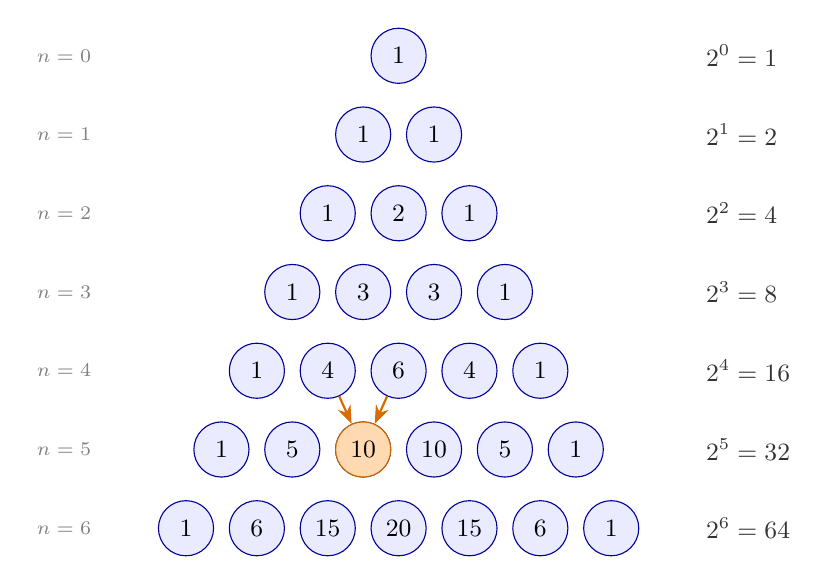
\begin{tikzpicture}[>={Stealth}, x=9mm, y=10mm,
    entry/.style={circle, draw=blue!60!black, fill=blue!8, minimum size=7mm, inner sep=0pt, font=\small}]
  \foreach \n in {0,...,6} {
    \foreach \k in {0,...,\n} {
      \pgfmathtruncatemacro\b{factorial(\n)/(factorial(\k)*factorial(\n-\k))}
      \node[entry] (p\n-\k) at (\k - \n/2, -\n) {\b};
    }
    \pgfmathtruncatemacro\s{2^\n}
    \node[anchor=west, font=\small, gray!40!black] at (4.2,-\n) {$2^{\n} = \s$};
  }
  % Row 5's 10 is row 4's 4 plus row 4's 6
  \foreach \u in {p4-1, p4-2} \draw[->, thick, orange!85!black] (\u) -- (p5-2);
  \node[entry, fill=orange!30, draw=orange!80!black] at (p5-2) {10};
  \foreach \n in {0,...,6} \node[anchor=east, font=\scriptsize, gray] at (-4.2,-\n) {$n = \n$};
\end{tikzpicture}
